\documentclass{article}
\usepackage{indentfirst}
\usepackage[utf8]{inputenc}
\usepackage[T1]{fontenc}
\usepackage[brazilian]{babel}
\usepackage{lmodern}
\usepackage{graphicx}
\usepackage{float}
\usepackage[]{subfigure}
\usepackage{afterpage}
\usepackage{amsmath}
\usepackage{textcomp,gensymb}
\usepackage{nameref}
\usepackage{accents}
\usepackage{listings}
\usepackage{color,soul}
\usepackage[margin=1in]{geometry}
\usepackage{steinmetz}

\PassOptionsToPackage{hyphens}{url}\usepackage{hyperref}
\hypersetup{
    breaklinks = true,
}
\urlstyle{same}
\newcommand{\ubar}[1]{\underaccent{\bar}{#1}}
%\renewcommand\thesection{\arabic{section}$^a$}
\renewcommand\thesection{\arabic{section}.}
\renewcommand\thesubsection{\arabic{section}.\alph{subsection}}
\definecolor{dkgreen}{rgb}{0,0.6,0}
\definecolor{gray}{rgb}{0.5,0.5,0.5}
\definecolor{mauve}{rgb}{0.58,0,0.82}
\lstset{
    frame=tb,
    language=Matlab,
    aboveskip=3mm,
    belowskip=3mm,
    showstringspaces=false,
    basicstyle={\small\ttfamily},
    numbers=none,
    numberstyle=\tiny\color{gray},
    keywordstyle=\color{blue},
    commentstyle=\color{dkgreen},
    stringstyle=\color{mauve},
    breaklines=true,
    breakatwhitespace=true,
    tabsize=4
}

\title{Simulação 3 - Controle Digital}
\author{Arthur de Matos Beggs - 12/0111098}
\date{2021}

\begin{document}
% capa
\begin{titlepage}
    \begin{center}
        \centering
        
\includegraphics[width=.7\linewidth]{images/logo_unb.png}\\[0.5cm]
        {\large \textbf{Universidade de Brasília}}\\[0.2cm]
        {\large \textbf{Departamento de Engenharia Elétrica}}\\[0.2cm]
        {\large \textbf{Controle Digital}}\\[4.8cm]
        {\bf \huge {Exercício de Simulação 3}}\\[0.2cm]
        {\bf \large {}}
    \end{center}

    \vspace{5cm}
    \hspace{2cm} {\noindent \bf \large {Aluno:}}\\
    \vspace{0.8cm}
    \hspace{2.35cm} {\large Arthur de Matos Beggs --------------------------------- 12/0111098}\\[1cm]

    \begin{center}
        {\large Brasília}\\
        {\large 2$^{\ubar{\circ}}$/2020}
    \end{center}

\end{titlepage}

\clearpage % Quebra de página

\setcounter{page}{2}


% \section{Questão 1}
%
%     \begin{figure}[H]
%        \centering
%             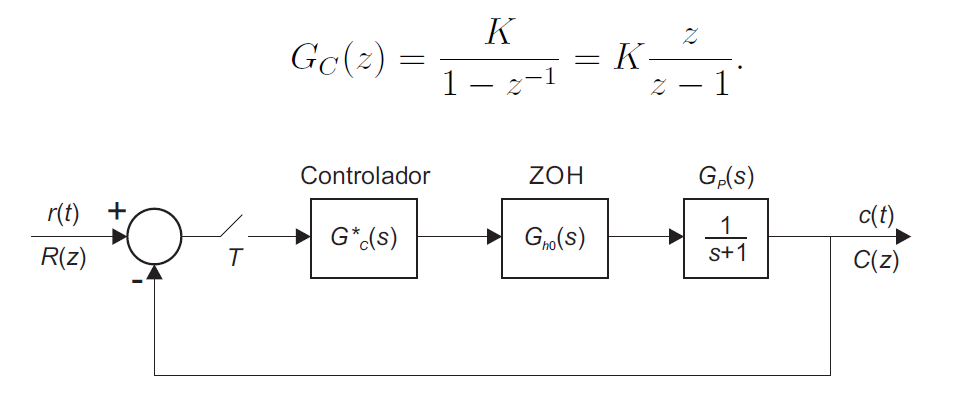
\includegraphics[width=1\linewidth]{images/Diagrama.png}
%             \caption{Diagrama e funções de transferência do sistema.}
%             \label{fig:diagram}
%     \end{figure}
%
%     {\textbf{a)} Para esboçar o LGR para os períodos de amostragem T = 0,5s, T = 1s e T = 2s, o seguinte script foi utilizado:}
%
% \vspace{7mm}
% \begin{lstlisting}
% s    = tf('s');
% Gp   = 1/(s+1);
%
% T1   = 0.5;
% z1   = tf('z',T1);
% Gc1  = z1/(z1-1);
% rl1  = c2d(Gp, T1, 'zoh') * Gc1;
%
% T2   = 1.0;
% z2   = tf('z',T2);
% Gc2  = z2/(z2-1);
% rl2  = c2d(Gp, T2, 'zoh') * Gc2;
%
% T3   = 2.0;
% z3   = tf('z',T3);
% Gc3  = z3/(z3-1);
% rl3  = c2d(Gp, T3, 'zoh') * Gc3;
%
% rlocus(rl1, rl2, rl3);
%
% \end{lstlisting}
%
%     \vspace{7mm}
%     {A execução do script gerou o \textit{plot} apresentado na Figura 2.}
%
%     \newpage
%
%     \begin{figure}[H]
%        \centering
%             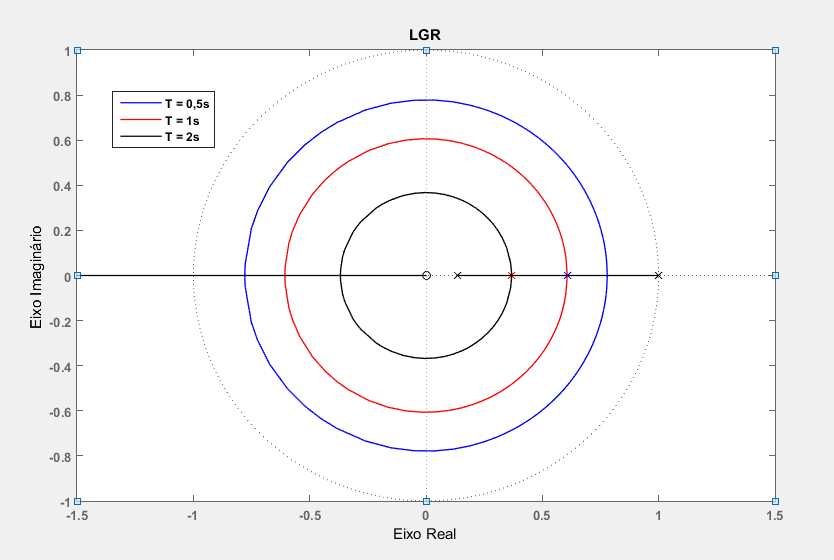
\includegraphics[width=1\linewidth]{images/LGR.png}
%             \caption{LGR no plano \textit{z} para T = 0,5s, 1s e 2s.}
%             \label{fig:lgr}
%     \end{figure}
%
%
%     \vspace{7mm}
%     {\textbf{b)} O valor de K crítico para cada período de amostragem é encontrado graficamente com o auxílio do cursor do Matlab no ponto em que o LGR deixa o círculo de raio unitário. A medida com o cursor apresenta uma imprecisão considerável, e por isso os valores de K crítico obtidos por esse método devem ser interpretados como aproximações.}
%
%     \vspace{7mm}
%     \begin{figure}[H]
%        \centering
%             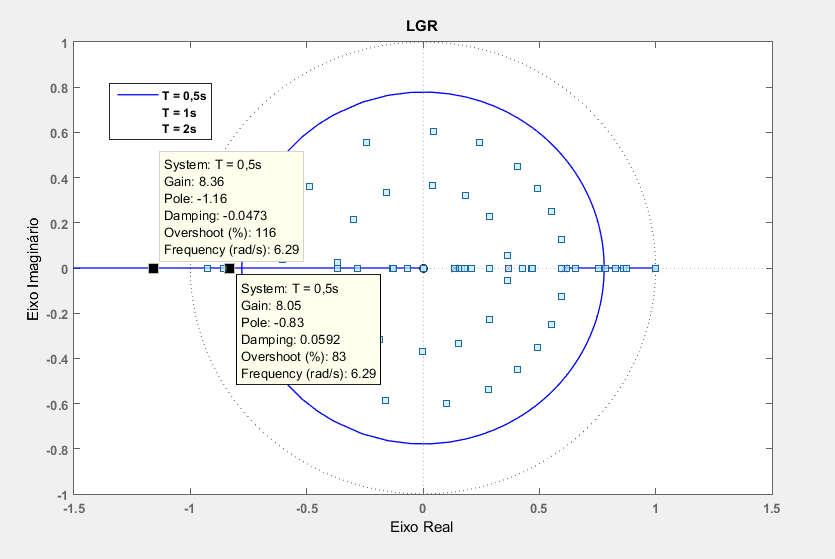
\includegraphics[width=.9\linewidth]{images/LGR_Kcrit05.png}
%             \caption{Para T = 0,5s, Kcrit $\approx$ 8,205 (obtido por interpolação).}
%             \label{fig:Kcrit05}
%     \end{figure}
%
%     \begin{figure}[H]
%        \centering
%             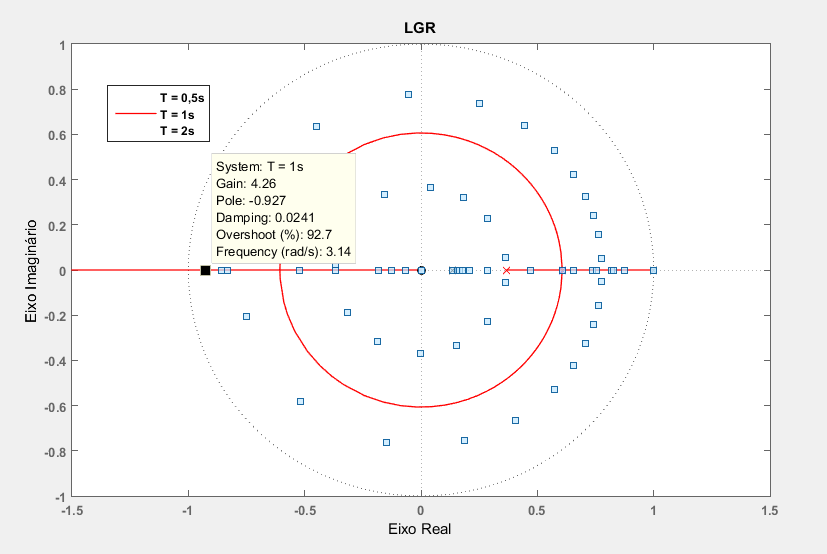
\includegraphics[width=1\linewidth]{images/LGR_Kcrit1.png}
%             \caption{Para T = 1s, Kcrit $\approx$ 4,26.}
%             \label{fig:Kcrit1}
%     \end{figure}
%
%     \begin{figure}[H]
%        \centering
%             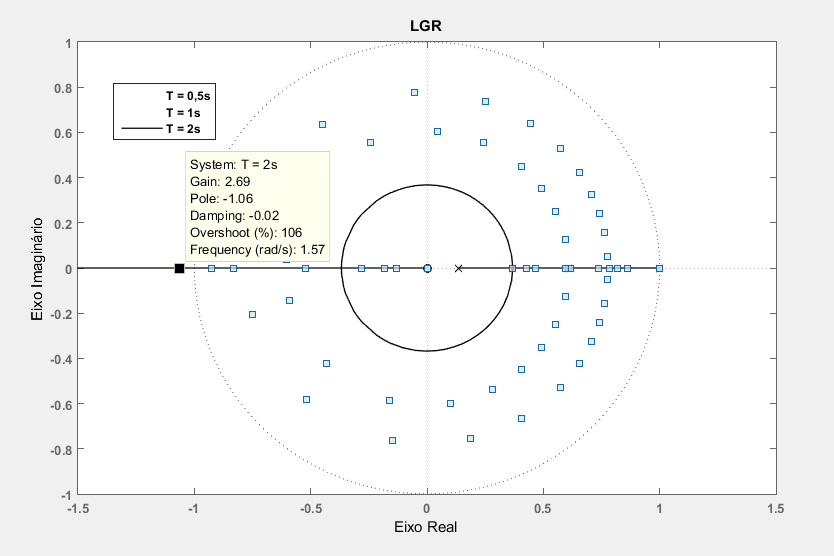
\includegraphics[width=1\linewidth]{images/LGR_Kcrit2.png}
%             \caption{Para T = 2s, Kcrit $\approx$ 2,69.}
%             \label{fig:Kcrit2}
%     \end{figure}
%
%     \clearpage
%
%     {\textbf{c)} Os pólos dominantes de malha fechada no plano \textit{z} quando K = 2 para cada valor de T foram obtidos posicionando o cursor sobre o ganho = 2. A medida com o cursor apresenta uma imprecisão considerável, e por isso os valores dos pólos dominantes obtidos por esse método devem ser interpretados como aproximações.}
%
%     \vspace{7mm}
%     \begin{figure}[H]
%        \centering
%             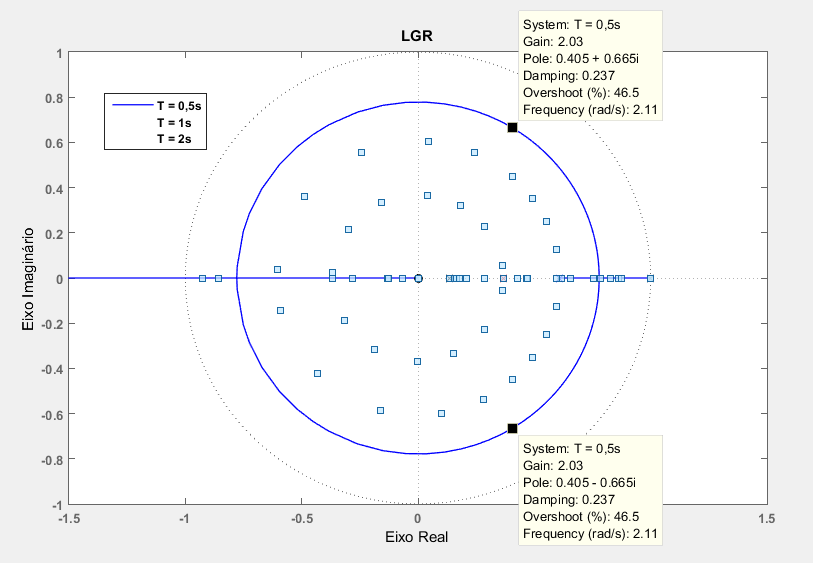
\includegraphics[width=.9\linewidth]{images/LGR_PoloDom05.png}
%             \caption{Para T = 0,5s, os pólos dominantes $\approx$ 0,405 $\pm$ 0,665j.}
%             \label{fig:poloDom05}
%     \end{figure}
%
%     \begin{figure}[H]
%        \centering
%             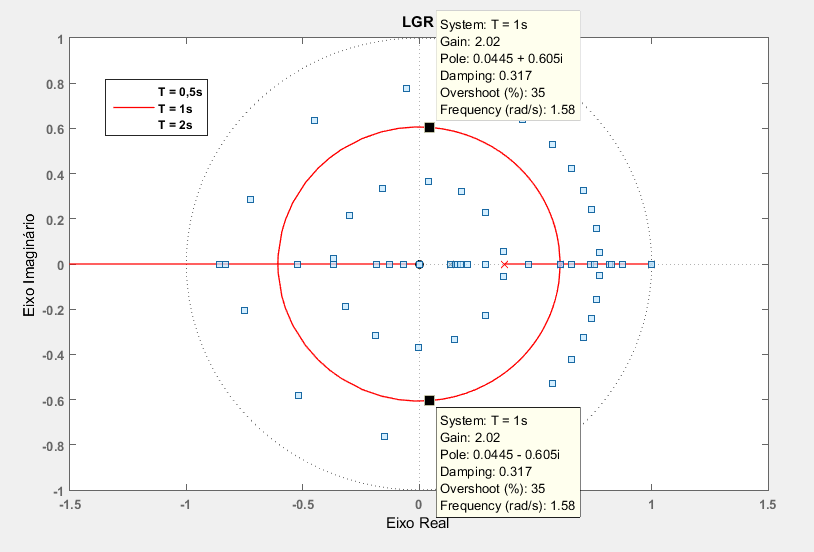
\includegraphics[width=.9\linewidth]{images/LGR_PoloDom1.png}
%             \caption{Para T = 1s, os pólos dominantes $\approx$ 0,0445 $\pm$ 0,605j.}
%             \label{fig:poloDom1}
%     \end{figure}
%
%     \begin{figure}[H]
%        \centering
%             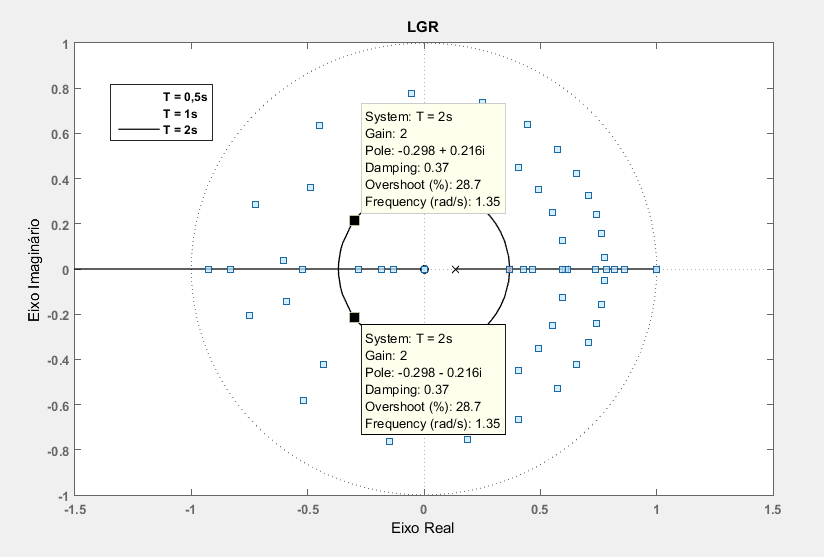
\includegraphics[width=1\linewidth]{images/LGR_PoloDom2.png}
%             \caption{Para T = 2s, os pólos dominantes $\approx$ -0,298 $\pm$ 0,216j.}
%             \label{fig:poloDom2}
%     \end{figure}
%
%
%     \vspace{7mm}
%     {Para as letras \textbf{d} e \textbf{e}, o diagrama do Simulink presente na Fig 9 foi utilizado.}
%
%     \begin{figure}[H]
%        \centering
%             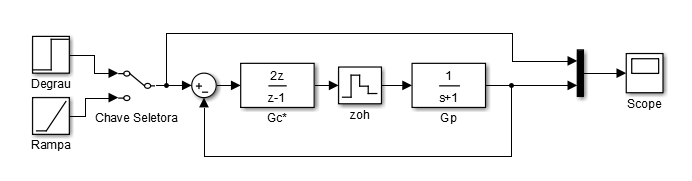
\includegraphics[width=1\linewidth]{images/DiagramaSimulink.png}
%             \caption{Diagrama do sistema representado no Simulink.}
%             \label{fig:diagSim}
%     \end{figure}
%
%     \vspace{14mm}
%     {\textbf{d)} As respostas ao degrau do sistema para diferentes tempos de amostragem e K = 2 são apresentadas nas figuras a seguir.}
%
%     \begin{figure}[H]
%        \centering
%             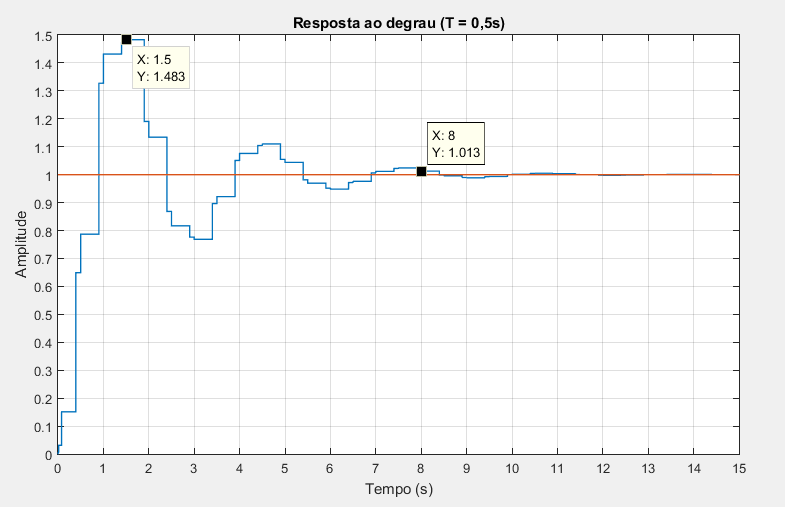
\includegraphics[width=1\linewidth]{images/rDeg05.png}
%             \caption{Resposta ao degrau unitário para T = 0,5s.}
%             \label{fig:rDeg05}
%     \end{figure}
%
%     {Para T = 0,5s, o sobressinal $\approx$  48,3\% e o tempo de acomodação $\approx$ 8 segundos.}
%
%     \vspace{7mm}
%     \begin{figure}[H]
%        \centering
%             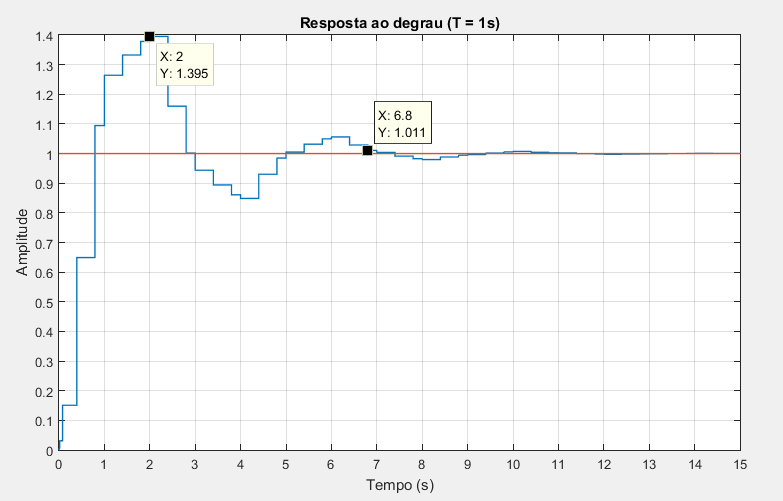
\includegraphics[width=1\linewidth]{images/rDeg1.png}
%             \caption{Resposta ao degrau unitário para T = 1s.}
%             \label{fig:rDeg1}
%     \end{figure}
%
%     {Para T = 1s, o sobressinal $\approx$ 39,5\% e o tempo de acomodação $\approx$ 6,8 segundos.}
%
%     \vspace{7mm}
%     \begin{figure}[H]
%        \centering
%             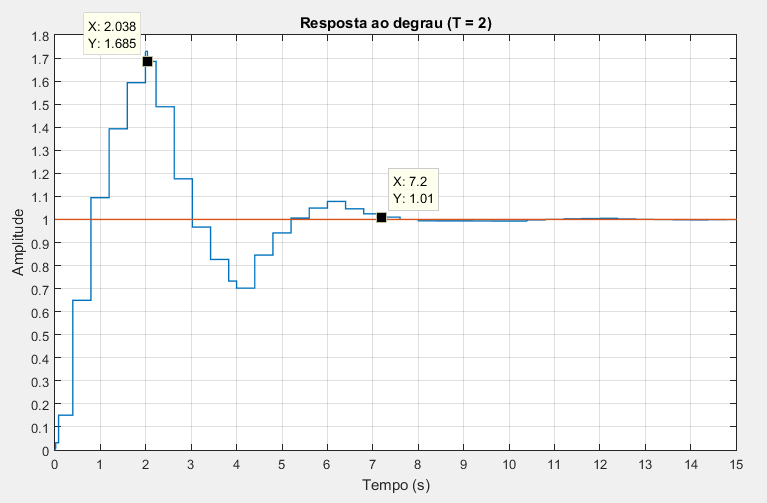
\includegraphics[width=1\linewidth]{images/rDeg2.png}
%             \caption{Resposta ao degrau unitário para T = 2s.}
%             \label{fig:rDeg2}
%     \end{figure}
%
%     {Para T = 2s, o sobressinal $\approx$ 68,5\% e o tempo de acomodação $\approx$ 7,2 segundos.}
%
%     \vspace{14mm}
%     {\textbf{e)} As respostas à rampa do sistema para diferentes tempos de amostragem e K = 2 são apresentadas nas figuras a seguir.}
%
%     \begin{figure}[H]
%        \centering
%             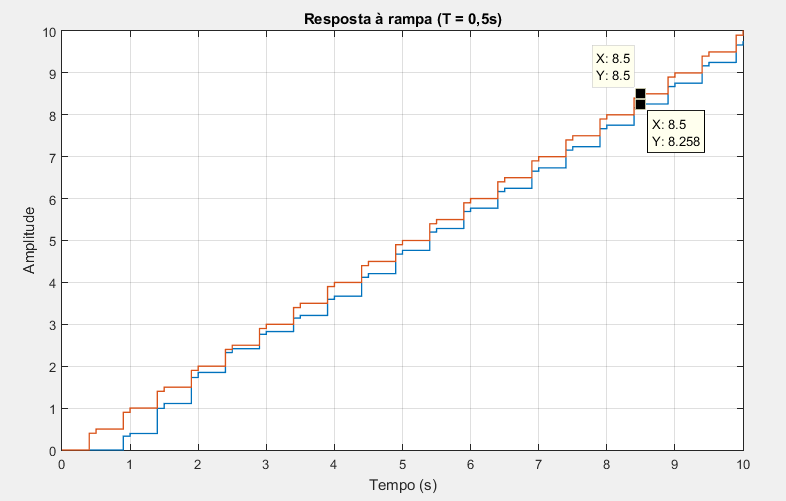
\includegraphics[width=1\linewidth]{images/rRamp05.png}
%             \caption{Resposta à rampa para T = 0,5s.}
%             \label{fig:rRamp05}
%     \end{figure}
%
%     {Para T = 0,5s, o erro em regime permanente Kv para uma entrada rampa $\approx$ 0,242.}
%
%     \vspace{7mm}
%     \begin{figure}[H]
%        \centering
%             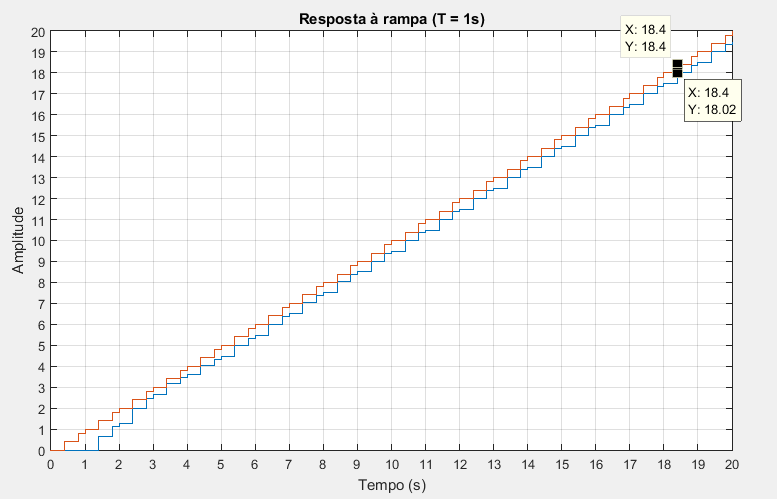
\includegraphics[width=1\linewidth]{images/rRamp1.png}
%             \caption{Resposta à rampa para T = 1s.}
%             \label{fig:rRamp1}
%     \end{figure}
%
%     {Para T = 1s, o erro em regime permanente Kv para uma entrada rampa $\approx$ 0,38.}
%
%     \vspace{7mm}
%     \begin{figure}[H]
%        \centering
%             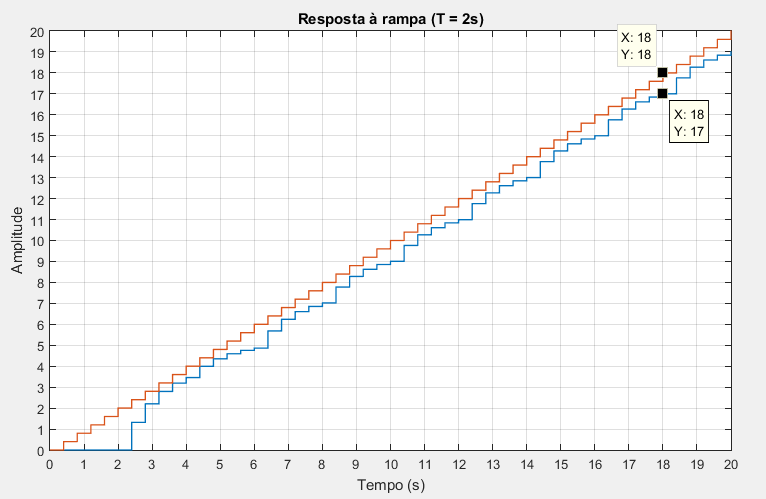
\includegraphics[width=1\linewidth]{images/rRamp2.png}
%             \caption{Resposta à rampa para T = 2s.}
%             \label{fig:rRamp2}
%     \end{figure}
%
%     {Para T = 2s, o erro em regime permanente Kv para uma entrada rampa $\approx$ 1.}
%
% %\newpage

%    \begin{figure}[H]
%       \centering
%            \includegraphics[width=1\linewidth]{images/.png}
%            \caption{}
%            \label{fig:}
%    \end{figure}

{\Large \bf Considere o sistema de controle a tempo discreto mostrado na
    Figura~\ref{fig:q2_diagrama}, cujo período de amostragem é $T = 0.2 s$.}

    \begin{figure}[H]
       \centering
            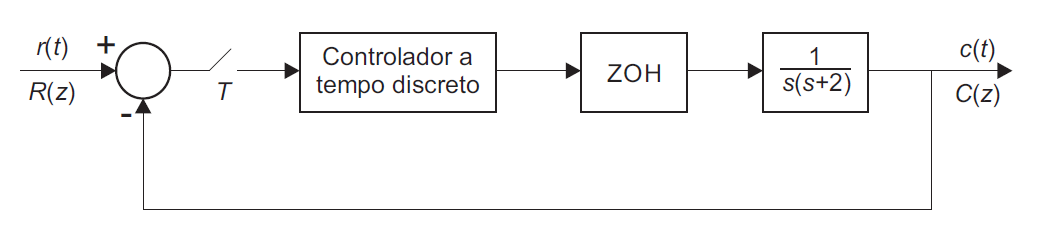
\includegraphics[width=1\linewidth]{images/q2_diagrama.png}
            \caption{Diagrama do sistema.}
            \label{fig:q2_diagrama}
    \end{figure}

    \section{Usando a técnica do LGR, projete no plano $z$ um controlador de
        modo que os polos dominantes de malha fechada tenham um fator de
        amortecimento $\zeta = 0.5$ e tempo de acomodação $t_s = 2\,s$:}

        \[ G_p(s) = G_{h0}(s) \times \frac{1}{s(s+2)} \]
        \[
            G_p(z) = \mathcal{Z}\left\{ G_{h0}(s) \times \frac{1}{s(s+2)} \right\}
                = (1-z^{-1}) \mathcal{Z}\left\{ \frac{1}{s^2 (s+2)} \right\}
        \]\\

        {Com o auxílio do Matlab,\\
        >> $T = 0.2;$\\
        >> $s = tf('s');$\\
        >> $z = tf('z', T);$\\
        >> $Gp\_s = zpk([\;], [0 \;\; -2], [1]);$\\
        >> $Gp\_z = c2d(Gp\_s, T, 'zoh')$ }\\

        \[ G_p(z) = \frac{0.01758(z+0.8753)}{(z-1)(z-0.6703)} \]\\

        {Temos que $t_s = \frac{4}{\zeta\omega_n}$, e dado que $t_s = 2\,s$ e
            $\zeta = 0.5$,}

        \[ \omega_n = \frac{4}{t_s\zeta} = 4 \,rad/s \]
        \[ \omega_d = \omega_n\sqrt{1-\zeta^2} = 3.4641 \,rad/s \]\\

        {Com $z = e^{sT} = e^{-\zeta\omega_nT}e^{j\omega_dT}$,}

        \[ |z| = e^{-\zeta\omega_nT} = 0.6703 \]
        \[ \angle z = \omega_dT = 39.6957^\circ \]\\

        {O par de polos complexos conjugados dominantes desejado pode ser
            encontrado por}

        \[ z_{dom} = |z|\left(\cos(\angle z) \pm j\sin(\angle z)\right) = 0.5158 \pm j0.4281 \]\\

        {O LGR do sistema não controlado apresentado na Figura~\ref{fig:q2_lgr_descontrolado}
            foi obtido no Matlab usando os comandos\\
        >> $ hold \; on $\\
        >> $ rlocus(Gp\_z) $\\
        >> $ plot(real(z\_dom),imag(z\_dom),'r*',real(z\_dom),-imag(z\_dom),'r*') $ }\\

        \begin{figure}[H]
           \centering
                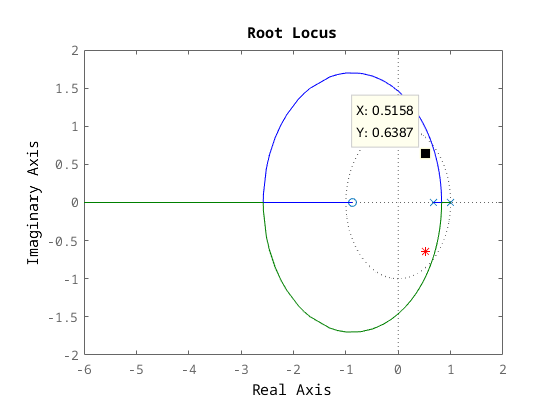
\includegraphics[width=1\linewidth]{images/q2_rlocus_uncontrolled.png}
                \caption{LGR do sistema $G_p(z)$, com os polos dominantes de
                    malha fechada representados por um asterisco vermelho e pelo
                    \textit{data cursor} do Matlab.}
                \label{fig:q2_lgr_descontrolado}
        \end{figure}

        {Pelo gráfico, o polo dominante desejado não faz parte do LGR do sistema.
            A condição de fase é utilizada para encontrar a contribuição angular
            que o controlador deve fornecer.}

        {O controlador projetado terá a forma $G_c(z) = K_c\frac{z - z_c}{z - p_c}$.

        {Como o a planta discretizada possui dois polos e um zero finito, o
            controlador fará o cancelamento do polo $z \neq 1$.}

        \[ \angle G_p(z) = \arctan\left( \frac{0.4281}{ 0.5158 + 0.8753 } \right)
                - \left(180^\circ - \arctan\left( \frac{0.4281}{ 1 - 0.5158 } \right) \right) \qquad\qquad\]
        \[\qquad\qquad\qquad\qquad - \left(180^\circ - \arctan\left( \frac{0.4281}{ 0.6703 - 0.5158 } \right) \right)
                + \left(180^\circ - \arctan\left( \frac{0.4281}{ 0.6703 - 0.5158 } \right) \right) \]\\
        \[ \angle G_p(z) = 121.4106^\circ \neq 180^\circ \pm 360^\circ i \]\\

        {Assim, o polo do controlador precisa contribuir com
        $180^\circ - 121.4106^\circ = 58.5893^\circ$.}

        \[ tan(58.5893^\circ) = \frac{0.4281}{ 0.5158 - p_c}
            \implies p_c = -\frac{0.4281}{tan(58.5893^\circ)} + 0.5158 = 0.2543 \]

        {O controlador projetado é dado por}
        \[ G_c(z) = K_c\frac{z - 0.6703}{z - 0.2543} \quad , \]
        {onde $K_c$ é o ganho do controlador.}

        {A função de transferência de malha aberta do sistema controlado é dada por}
        \[ G_s(z) = G_c(z) \times G_p(z) = \frac{0.01758K_c(z+0.8753)}{(z-1)(z-0.2543)} \]

        {O LGR do sistema $G_s(z)$ apresentado na Figura~\ref{fig:q2_lgr_controlled}
            foi obtido no Matlab usando os comandos\\
        >> $ Gc\_z = zpk([0.6703], [0.2543], [1], T); $\\
        >> $ Gs\_z = Gc\_z * Gp\_z $\\
        >> $ hold \; on $\\
        >> $ rlocus(Gs\_z) $\\
        >> $ plot(real(z\_dom),imag(z\_dom),'r*',real(z\_dom),-imag(z\_dom),'r*') $ }\\

        \begin{figure}[H]
           \centering
                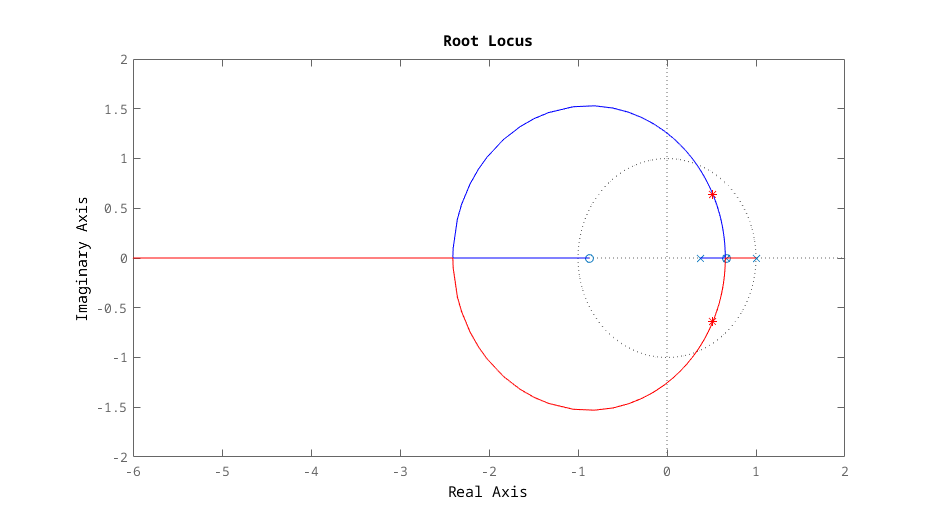
\includegraphics[width=1\linewidth]{images/q2_rlocus_controlled.png}
                \caption{LGR do sistema $G_s(z)$, com os polos dominantes de
                    malha fechada representados por asteriscos vermelhos
                    fazendo parte do LGR.}
                \label{fig:q2_lgr_controlled}
        \end{figure}

        {Para encontrar o ganho $K_c$ do controlador, a condição de módulo é
            utilizada. Assim,}
        \[ \left|G_s(z)|\right_{z= 0.5158 + j0.4281} = \frac{0.01758K_c \left|z + 0.8753|\right}{\left|z - 1|\right \left|z - 0.2543|\right} = 1 \]
        \[ \implies K_c = \left.\frac{\left|z - 1|\right \left|z - 0.2543|\right}{0.01758 \left|z + 0.8753|\right} \right|_{z= 0.5158 + j0.4281} = 12.6722 \]\\

        \[ G_c(z) = \frac{12.6722(z - 0.6703)}{(z - 0.2543)} ;
            \quad G_s(z) = \frac{0.22278(z+0.8753)}{(z-1)(z - 0.2543)} \]\\


    \section{Obtenha computacionalmente a resposta ao degrau unitário do sistema
        em malha fechada. Verifique se os requisitos de projeto foram satisfeitos:}

        {A resposta do sistema em malha fechada a uma entrada degrau unitário
            é apresentada na Figura~\ref{fig:q2_step_response}
            foi obtida no Matlab usando o comando\\
        >> $ step(feedback(Gs\_z, 1)) $ }\\

        \begin{figure}[H]
           \centering
                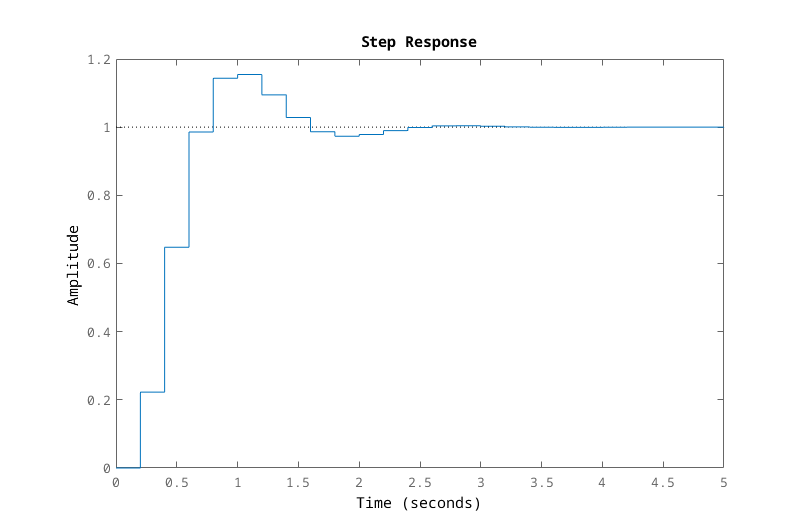
\includegraphics[width=1\linewidth]{images/q2_step_response.png}
                \caption{Resposta do sistema em malha fechada a uma entrada degrau unitário.}
                \label{fig:q2_step_response}
        \end{figure}

        {Os parâmetros da resposta foram obtidos pelo comando\\
        >> $ stepinfo(feedback(Gs\_z, 1)) $ }\\
        \begin{tabular}{ r l }
            RiseTime: & 0.400000000000000\\
            SettlingTime: & 2.200000000000000\\
            SettlingMin: & 0.973504789254130\\
            SettlingMax: & 1.154551426500324\\
            Overshoot: & 15.455142650032405\\
            Undershoot: & 0\\
            Peak: & 1.154551426500324\\
            PeakTime: & 1\\
        \end{tabular}\\

        {Verificando os parâmetros de resposta, o tempo de acomodação $t_s$ foi
            de $2.2\,s$, apenas um período de amostragem além do desejado.}
        {Para verificar se o requisito do coeficiente de amortecimento
            $\zeta = 0.5$ foi atendido, o \textit{overshoot} será utilizado.}

        \[ \zeta = \frac{-\log\left( \frac{\text{overshoot}}{100} \right)}{ \sqrt{ \pi^2 + \log^2\left( \frac{\text{overshoot}}{100} \right) } }
            = \frac{-\log\left( \frac{15.4551}{100} \right)}{ \sqrt{ \pi^2 + \log^2\left( \frac{15.4551}{100} \right) } }
            = 0.5109 \]\\

        {O resultado do projeto se aproxima satisfatoriamente dos requisitos.}


    \section{Obtenha computacionalmente a resposta à rampa unitária do sistema
        em malha fechada. Determine o valor do erro estacionário:}

        {A resposta do sistema em malha fechada a uma entrada rampa unitária
            apresentada na Figura~\ref{fig:q2_ramp_response} e seus dados brutos
            foram obtidos pelos comandos\\
        >> $ time = (0:T:10); $\\
        >> $ ramp\_output = lsim(feedback(Gs\_z, 1), time, time); $\\
        >> $ lsim(feedback(Gs\_z, 1), time, time) $ }\\

        \begin{figure}[H]
           \centering
                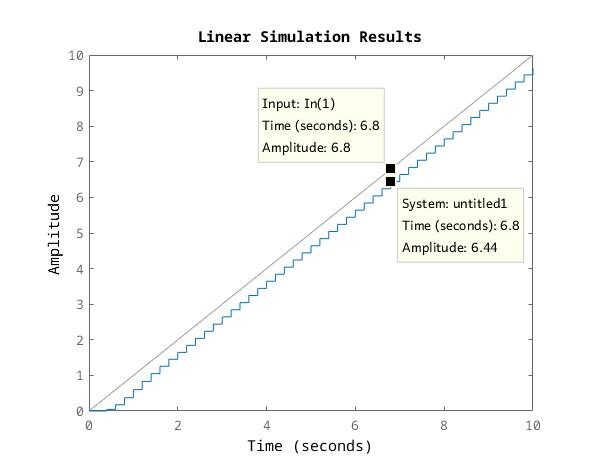
\includegraphics[width=1\linewidth]{images/q2_ramp_response.png}
                \caption{Resposta do sistema em malha fechada a uma entrada rampa unitária.}
                \label{fig:q2_ramp_response}
        \end{figure}

        {O erro estacionário $e_{ss}$ pode ser encontrado por}\\
        \[ e_{ss} = \lim\limits_{z \to 1} (1 - z^{-1}) \frac{1}{1 + G_s(z)}
                \times \frac{Tz^{-1}}{(1- z^{-1})^2 }
                = \frac{1}{K_v} \]
        \[ K_v = \frac{1}{T} \lim\limits_{z \to 1} (1-z^{-1}) G_s(z)
            =   \frac{1}{T} \lim\limits_{z \to 1} (1-z^{-1})
            \times \frac{0.22278(z+0.8753)}{(z-1)(z - 0.2543)} \]
        \[ K_v = 2.8012; \quad e_{ss} = \frac{1}{K_v} = 0.3569 \]

        {Para obter computacionalmente o erro estacionário, o período anterior
            ao tempo de acomodação foi ignorado, e foi tomada a média das
            diferenças entre o sinal da rampa unitária e o sinal de saída do sistema.\\
        >> $ time\_slice = time((step\_info.SettlingTime/T):end); $\\
        >> $ ramp\_slice = ramp\_output((step\_info.SettlingTime/T):end); $\\
        >> $ e\_ss = mean(arrayfun(@(x,y) x - y, time\_slice, ramp\_slice.')) $ }\\

        {Assim, o erro estacionário encontrado computacionalmente é
            $e_{ss} = 0.3569$, correspondendo ao valor calculado.}

    \section{Refaça o projeto de modo que o valor do erro estacionário seja
        reduzido a um terço do valor anterior e fazendo o LGR passar próximo dos
        polos dominantes usados no item $(1)$. Obtenha computacionalmente a
        resposta à rampa unitária do sistema em malha fechada. Verifique se o
        requisito do erro estacionário foi atingido. Obtenha computacionalmente
        a resposta ao degrau unitário do sistema em malha fechada. A resposta
        transitória foi semelhante à do item $(1)$? Explique a diferença:}

        {Para diminuir o erro estacionáro $e_{ss}$ em um terço, é necessário que
            a constante $K_v$ seja triplicada. Uma maneira de fazer isso é
            adicionar um polo e um zero ao controlador com valores próximos um
            do outro para ter uma contribuição de fase negligenciável, próximos
            de $z = 1$ e com valores onde $\lim\limits_{z \to 1}
            \frac{(z - z_v)}{(z - p_v)} = 3$. Escolhendo}
        \[ G_{c_2}(z) = G_c(z) \frac{(z - 0.94)}{(z - 0.98)} \]
        \[ K_v = \frac{1}{T} \lim\limits_{z \to 1} (1-z^{-1})
            \times \frac{0.22278(z+0.8753)}{(z-1)(z - 0.2543)}
            \times \frac{(z - 0.94)}{(z - 0.98)}
            = 8.4037\]
        \[ e_{ss} = \frac{1}{K_v} = 0.11899 \]\\

        {O LGR com o novo controlador do sistema $G_s(z)$ apresentado na
        Figura~\ref{fig:q2_lgr_quicker} foi obtido no Matlab usando os comandos\\
        >> $ Gc2\_z = Gc\_z * zpk([0.94], [0.98], [1], T); $\\
        >> $ hold \; on $\\
        >> $ rlocus(Gp\_z * Gc2\_z) $\\
        >> $ plot(real(z\_dom),imag(z\_dom),'r*',real(z\_dom),-imag(z\_dom),'r*') $ }\\

        \begin{figure}[H]
           \centering
                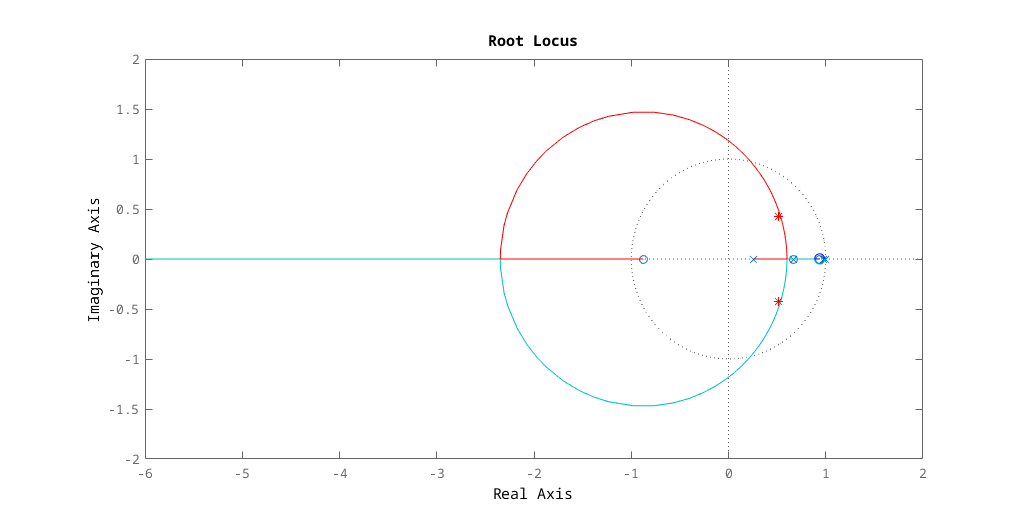
\includegraphics[width=.8\linewidth]{images/q2_rlocus_quicker.png}
                \caption{LGR do sistema $G_p(z)G_{c_2}(z)$, com os polos
                    dominantes de malha fechada representados por asteriscos
                    vermelhos bem próximos do LGR.}
                \label{fig:q2_lgr_quicker}
        \end{figure}

        {Os polos dominantes de malha fechada ficam muito próximos do LGR com
            o novo controlador. A resposta à rampa unitária apresentada na
            Figura~\ref{fig:q2_ramp_response_new} e seus dados brutos foram obtidos
            pelos comandos\\
        >> $ time = (0:T:10); $\\
        >> $ lsim(feedback(Gp\_z * Gc2\_z, 1), time, time) $\\
        >> $ \text{\% tempo maior p/ melhorar média} $\\
        >> $ time\_longer = (0:T:25); $\\
        >> $ ramp\_output\_new = lsim(feedback(Gp\_z * Gc2\_z, 1), time\_longer, time\_longer); $ }\\

        \begin{figure}[H]
           \centering
                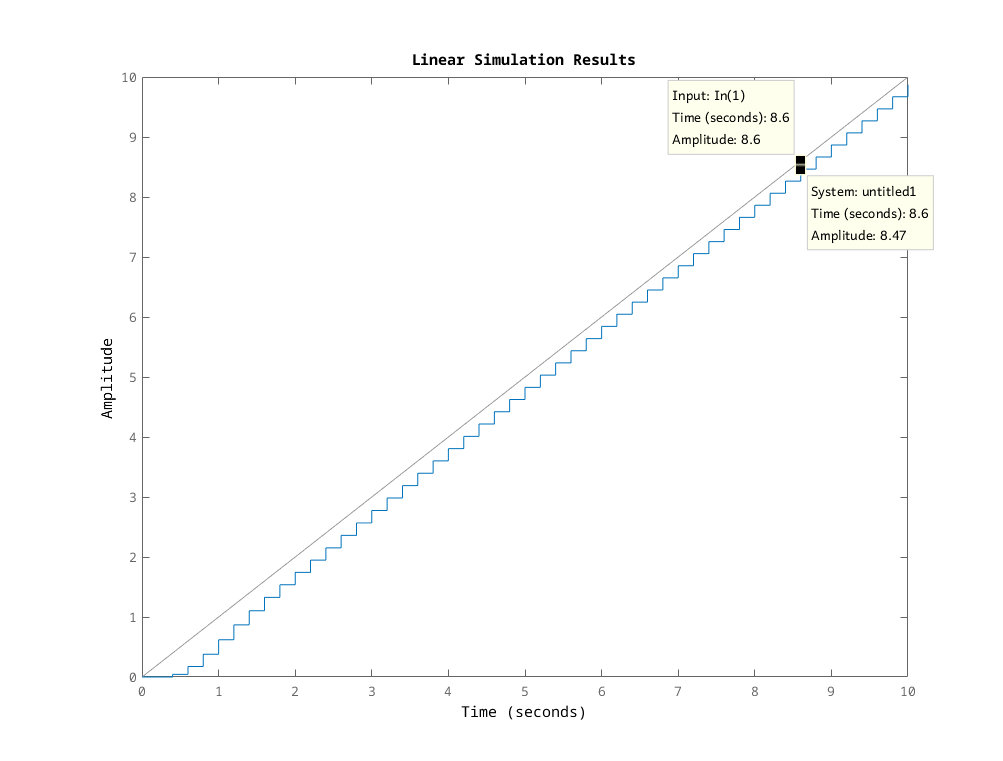
\includegraphics[width=.8\linewidth]{images/q2_ramp_response_new.png}
                \caption{Resposta do sistema com novo controlador em malha
                    fechada a uma entrada rampa unitária.}
                \label{fig:q2_ramp_response_new}
        \end{figure}

        {Pelos \textit{data cursors} o valor do erro estacionário da resposta
            a uma entrada rampa unitária parece próximo do desejado. A
            Figura~\ref{fig:q2_step_response_new} mostra a nova resposta do sistema
            a uma entrada degrau unitário. O gráfico e os parâmetros da resposta
            foram obtidos usando os comandos\\
        >> $ step(feedback(Gp\_z * Gc2\_z, 1)) $\\
        >> $ stepinfo(feedback(Gp\_z * Gc2\_z, 1)) $ }\\

        \begin{figure}[H]
           \centering
                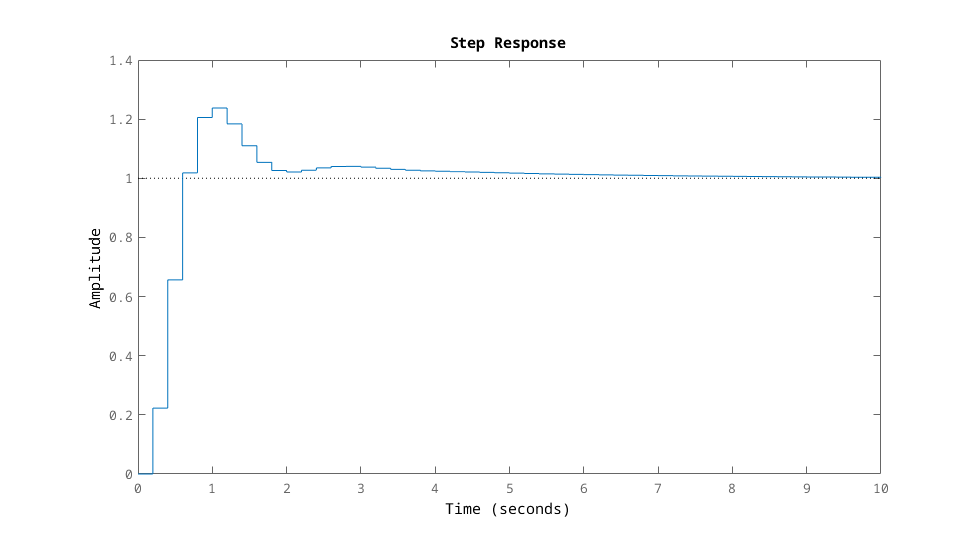
\includegraphics[width=1\linewidth]{images/q2_step_response_new.png}
                \caption{Resposta do sistema com novo controlador em malha
                    fechada a uma entrada degrau unitário.}
                \label{fig:q2_step_response_new}
        \end{figure}

        \begin{tabular}{ r l }
            RiseTime:& 0.400000000000000\\
            SettlingTime:& 4.600000000000001\\
            SettlingMin:& 1.000235449277402\\
            SettlingMax:& 1.237606634699172\\
            Overshoot:& 23.760663469918232\\
            Undershoot:& 0\\
            Peak:& 1.237606634699172\\
            PeakTime:& 1\\
        \end{tabular}\\

        {Pelos valores obtidos para a resposta degrau, o tempo de acomodação
            mais que dobrou, não obedecendo o requisito de projeto de $t_s =2\,s$.
            Calculando o coeficiente de amortecimento $\zeta$ a partir do
            \textit{Overshoot},}
        \[ \zeta = \frac{-\log\left( \frac{\text{overshoot}}{100} \right)}{ \sqrt{ \pi^2 + \log^2\left( \frac{\text{overshoot}}{100} \right) } }
            = \frac{-\log\left( \frac{23.7606}{100} \right)}{ \sqrt{ \pi^2 + \log^2\left( \frac{23.7606}{100} \right) } }
            = 0.41599 \]\\

        {Assim, o requisito de $\zeta = 0.5$ também não é respeitado no novo
            controlador.}\\

        {Para obter computacionalmente o erro estacionário, o período anterior
            ao tempo de acomodação foi ignorado, e foi tomada a média das
            diferenças entre o sinal da rampa unitária e o sinal de saída do sistema.\\
        >> $ time\_slice\_new = time((step\_info\_new.SettlingTime/T):end); $\\
        >> $ ramp\_slice\_new = ramp\_output((step\_info\_new.SettlingTime/T):end); $\\
        >> $ e\_ss\_new = mean(arrayfun(@(x,y) x - y, time\_slice\_new, ramp\_slice\_new.')) $ }\\

        {Assim, o erro estacionário encontrado computacionalmente é
            $e_{ss} = 0.1216$, próximo ao valor calculado de $0.11899$.}

        {Com o novo controlador, o erro estacionário para uma entrada rampa foi
            diminuído a quase $^1/_3$ do erro apresentado com o controlador
            original. Porém, o tempo de resposta aumentou consideravelmente,
            sendo mais que o dobro do obtido no controlador anterior. O coeficiente
            de amortecimento obtido tabmém foi mais baixo, resultando em um
            \textit{overshoot} maior.}

        {O script completo utilizado na simulação é apresentado a seguir:}
\begin{lstlisting}
% Parte 1
T = 0.2;
s = tf('s');
z = tf('z', T);
Gp_s = zpk([ ], [0 -2], [1]);
Gp_z = c2d(Gp_s, T, 'zoh')

zeta = 0.5;
t_s = 2;
j = sqrt(-1);
omega_n = 4/(zeta * t_s)
omega_d = omega_n * sqrt(1 - zeta^2)
mod_z = exp(-zeta * omega_n * T)
angle_z = rad2deg(omega_d * T)
z_dom = mod_z * cosd(angle_z) + j * mod_z * sind(angle_z)

% Root locus e polos dominantes
hold on;
rlocus(Gp_z)
plot(real(z_dom),imag(z_dom),'r*',real(z_dom),-imag(z_dom),'r*')
hold off;

% Condiçao de fase
[Z_dom, P_dom, K_dom] = zpkdata(Gp_z, 'v');
% Generalizar
controller_angle = -180 -( atand(imag(z_dom)/(max(real(z_dom),Z_dom(1)) - min(real(z_dom),Z_dom(1)))) -(180 - atand(imag(z_dom)/(max(real(z_dom),P_dom(1)) - min(real(z_dom),P_dom(1))))) )

p_c = (imag(z_dom)/tand(controller_angle)) + real(z_dom)
Gc_z = zpk([ P_dom(2) ], [p_c], [1], T)
Gs_z = Gc_z * Gp_z

% Root locus e polos dominantes
hold on;
rlocus(Gs_z,(0:0.01:100))
plot(real(z_dom),imag(z_dom),'r*',real(z_dom),-imag(z_dom),'r*')
hold off;

% Encontrando Kc
[Z_sys, P_sys, K_sys] = zpkdata(Gs_z, 'v');
Kc = ( abs(z_dom - P_sys(1)) * abs(z_dom - P_sys(2)) ) / ( K_sys * abs(z_dom - Z_sys(2)) )
Gc_z = Kc * Gc_z
Gs_z = Gc_z * Gp_z


% Parte 2
step(feedback(Gs_z, 1))
step_info = stepinfo(feedback(Gs_z, 1))
ts_response = step_info(1).SettlingTime;
zeta_response = (-log(step_info(1).Overshoot/100)/sqrt(pi^2 + log(step_info(1).Overshoot/100).^2))


% Parte 3
time = (0:T:10);
ramp_output = lsim(feedback(Gs_z, 1), time, time);

lsim(feedback(Gs_z, 1), time, time)

% Retira as amostras antes do tempo de acomodaçao
time_slice = time((step_info.SettlingTime/T):end);
ramp_slice = ramp_output((step_info.SettlingTime/T):end);
e_ss = mean(arrayfun(@(x,y) x - y, time_slice, ramp_slice.'))

% Cálculo do e_ss
syms z;
[Num_Gs, Den_Gs] = tfdata(Gs_z);
symbolic_Gs_z = vpa(poly2sym(cell2mat(Num_Gs),z)/poly2sym(cell2mat(Den_Gs),z));
z = 0.99999999999; % Poor man's limit
Kv = subs(collect(1/T * (z-1)/z * symbolic_Gs_z))
e_ss_calculated = 1/Kv

% Consertando z
z = tf('z', T);


% Parte 4
Gc2_z = Gc_z * zpk([0.94], [0.98], [1], T)

hold on;
rlocus(Gp_z*Gc2_z)
plot(real(z_dom),imag(z_dom),'r*',real(z_dom),-imag(z_dom),'r*')
hold off;

lsim(feedback(Gp_z*Gc2_z, 1), time, time)

time_longer = (0:T:25);
ramp_output_new = lsim(feedback(Gp_z*Gc2_z, 1), time_longer, time_longer);

step(feedback(Gp_z*Gc2_z, 1))

step_info_new = stepinfo(feedback(Gp_z*Gc2_z, 1))
ts_response_new = step_info_new(1).SettlingTime;
zeta_response_new = (-log(step_info_new(1).Overshoot/100)/sqrt(pi^2 + log(step_info_new(1).Overshoot/100).^2))

time_slice_new = time_longer((step_info_new.SettlingTime/T):end);
ramp_slice_new = ramp_output_new((step_info_new.SettlingTime/T):end);
e_ss_new = mean(arrayfun(@(x,y) x - y, time_slice_new, ramp_slice_new.'))

\end{lstlisting}

\end{document}

